\RequirePackage{snapshot}
\documentclass [10pt, fancyhdr, twoside] {article}
\usepackage{float, graphicx, caption, amssymb, natbib}
\usepackage[usenames,dvipsnames]{color}
\usepackage{tabulary}
\usepackage [left=2.5cm, top=2.5cm, bottom=2.5cm, right=3cm] {geometry}  %% see geometry.pdf on how to lay out the page. There's lots.
\geometry{a4paper} %% or letter or a5paper or ... etc
\usepackage{fancyhdr}
\usepackage{enumitem}
\usepackage{blindtext}
\usepackage{bbding}
\usepackage{tikz}
\usepackage{xcolor}
\usepackage{sectsty}
\usepackage[scaled]{helvet}
\renewcommand*\familydefault{\sfdefault} %% Only if the base font of the document is to be sans serif

\usepackage[left]{lineno}
\usepackage[yyyymmdd,hhmmss]{datetime}

\renewcommand{\linenumberfont}{\normalfont\tiny\color{gray}}

\pagestyle{fancy}

%\fancyhead{}
%\fancyfoot{}

%\fancyhead[RO,LE]{Heading}
%\fancyfoot[RO,LE]{}
%\fancyfoot[C]{Strana \thepage}
%\fancyfoot[RE, LO]{}

\sectionfont{\centering}
\subsectionfont{\centering}
\setcounter{secnumdepth}{0}

\newcounter {note}
\stepcounter{note}

\renewcommand{\abstractname}{Abstract Name}

\newcommand {\Note} [1] {
    \marginpar {
        \tiny {
            {\color{gray}{\thenote  \  #1}}
            }
        }
    \stepcounter {note}
}

\newcommand {\MNote} [1] {
    \marginpar {
        \tiny {
            {\color{gray}{#1 }}
            }
        }
}

\begin{document}

\title{Analýza výrobního programu \\
  \large Metodou \textsc{saturace hrubého rozpětí} \\
}

\author{
  Ing. Karel Hubálek, CSc.
  \and
  RNDr. Edvard Špaček
}
\date{}

\maketitle


% \linenumbers


\begin{itemize}[label=\EightFlowerPetalRemoved]
\item Chcete znát východisko ze své nepříznivé platební a obchodní situace?
\item Sestavte svůj výrobní program metodou \textsc{Saturace hrubého rozpětí}.
\item Tato metoda aplikačně proveřená vám zodopoví otázku jaký je váš stávající výrobní program, jaké má slabé a silné stránky, čím a s jakými ekonomickými parametry ho doplnit.
\item Výhoda metrody je, že se neorientuje pouze na ziskovou produkci a neutlumuje výrobu!
\item Metoda využívá stávající datovou základnu podniku, je datově nenáročná a dává přesvědčivé výsledky.
\item Je k dispozici program pro PC.
\end{itemize}


\section{Problémy}

V odbytových obtížích stojí řada podniků před obtížným rozhodnutím, mohu-li si dovolit zařadit do výrobního programu i ty akce, které sice ještě uhradí přímé výrobní náklady jako je materiál a mzdy, ale nezbyde už dost na složku celopodnikové režie. Budou-li \textbf{přínosy} z ostatních akcí pokrývat \textbf{očekávané minimalizované celopodnikové režijní náklady}, mohou se do výrobní strategie volit i \textbf{ztrátové programy}.

Pro tvorbu celopodnikového zisku nerozhoduje velikost kalkulovaných ziskovostí jednotlivých výrobků, ale rozdíl mezi realizovanými celopodnikovými příjmy a výdaji.

Náklady má podnik \textbf{přímé} - úměrné realizovaným výkonům a nepřímé - na těchto výkonech prakticky nezávislé. Nerealizuje-li se část produkce, pro níž byla ale v bilanci nákladovosti výrobků režijní složka započítána, musí se uhradit nejprve všechny náklady podniku, i nepřímé a teprve potom je možno realizovat zisk.

Takovýto globální přehled na oblast podnikového hospodaření je uplatněn v modelu \textbf{Saturace hrubého rozpětí}. Hrubé rozpětí zahrnuje v jedné položce nepřímé náklady i zisk.

Hrubé rozpětí výrobku stanovíme jako \textbf{rozdíl mezi cenou}, kterou výrobce za něj realizuje \textbf{a přímými náklady} na tento výrobek.


\section{Řešení}

Podnikové hrubé rozpětí naopak můžeme dobře bilancovat. Jsou to nepřímé náklady podnikových útvarů i odpisy základních prostředků. Lze stanovit i minimální výši bilančního zisku např. pomocí požadovaného procenta rentability výrobních fondů. Víme tedy, jakou celkovou částku bychom jednotlivými hrubými rozpětími výrobků \textbf{saturovat}, abychom docílili minimálního bilančního zisku. Setřídění výrobního programu, dle poměru hrubého rozpětí k pracnosti, ukáže výhodnost sortimentu a zodpoví:

\begin{itemize}
\item Jaký je výsledný reálný celopodnikový zisk.
\item Jak je zaplněna bilancovaná kapacita podniku.
\item Jak dalece je možné zařadit do výroby i akce s negativním kalkulovaným ziskem.
\end{itemize}

Model saturace hrubého rozpětí (obr. 1) je diagram závislosti mezi hrubým rozpětím a kapacitou v normohodinách. Bilancovaná kapacita podniku je zadána. Tato hodnota je užita při rozpočtu výrobní režie v kalkulaci cen výrobků. Jsou sledovány hodnoty \textbf{kalkulované} za celý podnik a \textbf{marketingem} docilované za jednotlivé složky výrobního programu.

Kalkulované, celopodnikové hodnoty jsou vyznačeny přímkami. Vodorovné jsou ve výši podnikového hrubého rozpětí HR, z toho je odečten bilanční zisk Z a odpisy O. Svislice znační kapacitu K.

Marketingem plánované, nebo už realizované údaje znázorňuje \textbf{saturační křivka}. Složky saturačního programu se tu řadí zpravidla podle podílu saturace hrubého rozpětí na kapacitě (směrinice saturační křivky), nebo i podle jiných kritérií, např. oborů, pracovišť a pod. Předpokládá se, že marketing dodá \textbf{zdrojový zásobník} možného výrobního programu s co nejvhodnějšími složkami, které ale mohou být v závislosti na odbytových možnostech v některých položkách i se ztrátovým bilančním ziskem. Saturační křivka pak na prvý pohled charakterizuje ekonomické možnosti výrobního programu.

V modelu saturace na obr. 1 jsou dále znázorněny:

\begin{itemize}
\item kumulovaný bilanční zisk a
\item měrný bilanční zisk na normohodinu pro jednotlivé akce.
\end{itemize}

Z podkladů jsou zpracovány \textbf{tabulkové Výpisy} jednotlivých programů i celého podniku - viz tab. 1 a 2. Nedoplněná kapacita podniku volá po zařazení doplňkového výrobního programu marketingem. Ten by musel realizovat směrnici saturační křivky v minimální výši dané diferencemi v plnění hrubého rozpětí a normohodin.

Sledování hlavních parametrů výrobního programu z hlediska saturace hrubého rozpětí se koncentruje do vyčíslování pěti kriteriálních ukazatelů sledovaných ze tří hledisek a do jednoho výsledného ukazatele, kterým je Podnikový zisk reálný PZR. Tyto ukazatele jsou obsaženy ve výstupní sestavě Analýza výrobního programu viz tab. 3. Její trojrozměrné zobrazení je na obr. 2.

Z tabulky vyplývá, že se uvedené ukazatele sledují ze tří hledisek:

\begin{itemize}
\item K – kalkulace, tj. údaje bilancované pro kalkulační vzorec, ty představují požadovaný normativ.
\item M – marketing, tedy údaje plánu navrhované obchodnímy útvary
\item D – diference, které představují nutný doplněk výrobního programu, aby byly splněny jeho kalkulované normativy.
\end{itemize}

Z výsledků v tabulkách a grafech vyplývají následující závěry:

\begin{itemize}
\item Plán podniku dává nebo nedává předpoklady pro docilování reálného požadovaného zisku PZR.
\item Lze vymezit oblasti, které dosahují záporné bilance, zejména pro reální zisk či dokonce záporný marketingový bilanční zisk.
\item Naproti tomu separovat oblasti dosahující nadprůměrného zisku.
\item Prověřit kapacitu v NH podle plánu MNH a provonat s kalkulovanou KNH.
\end{itemize}


\newpage

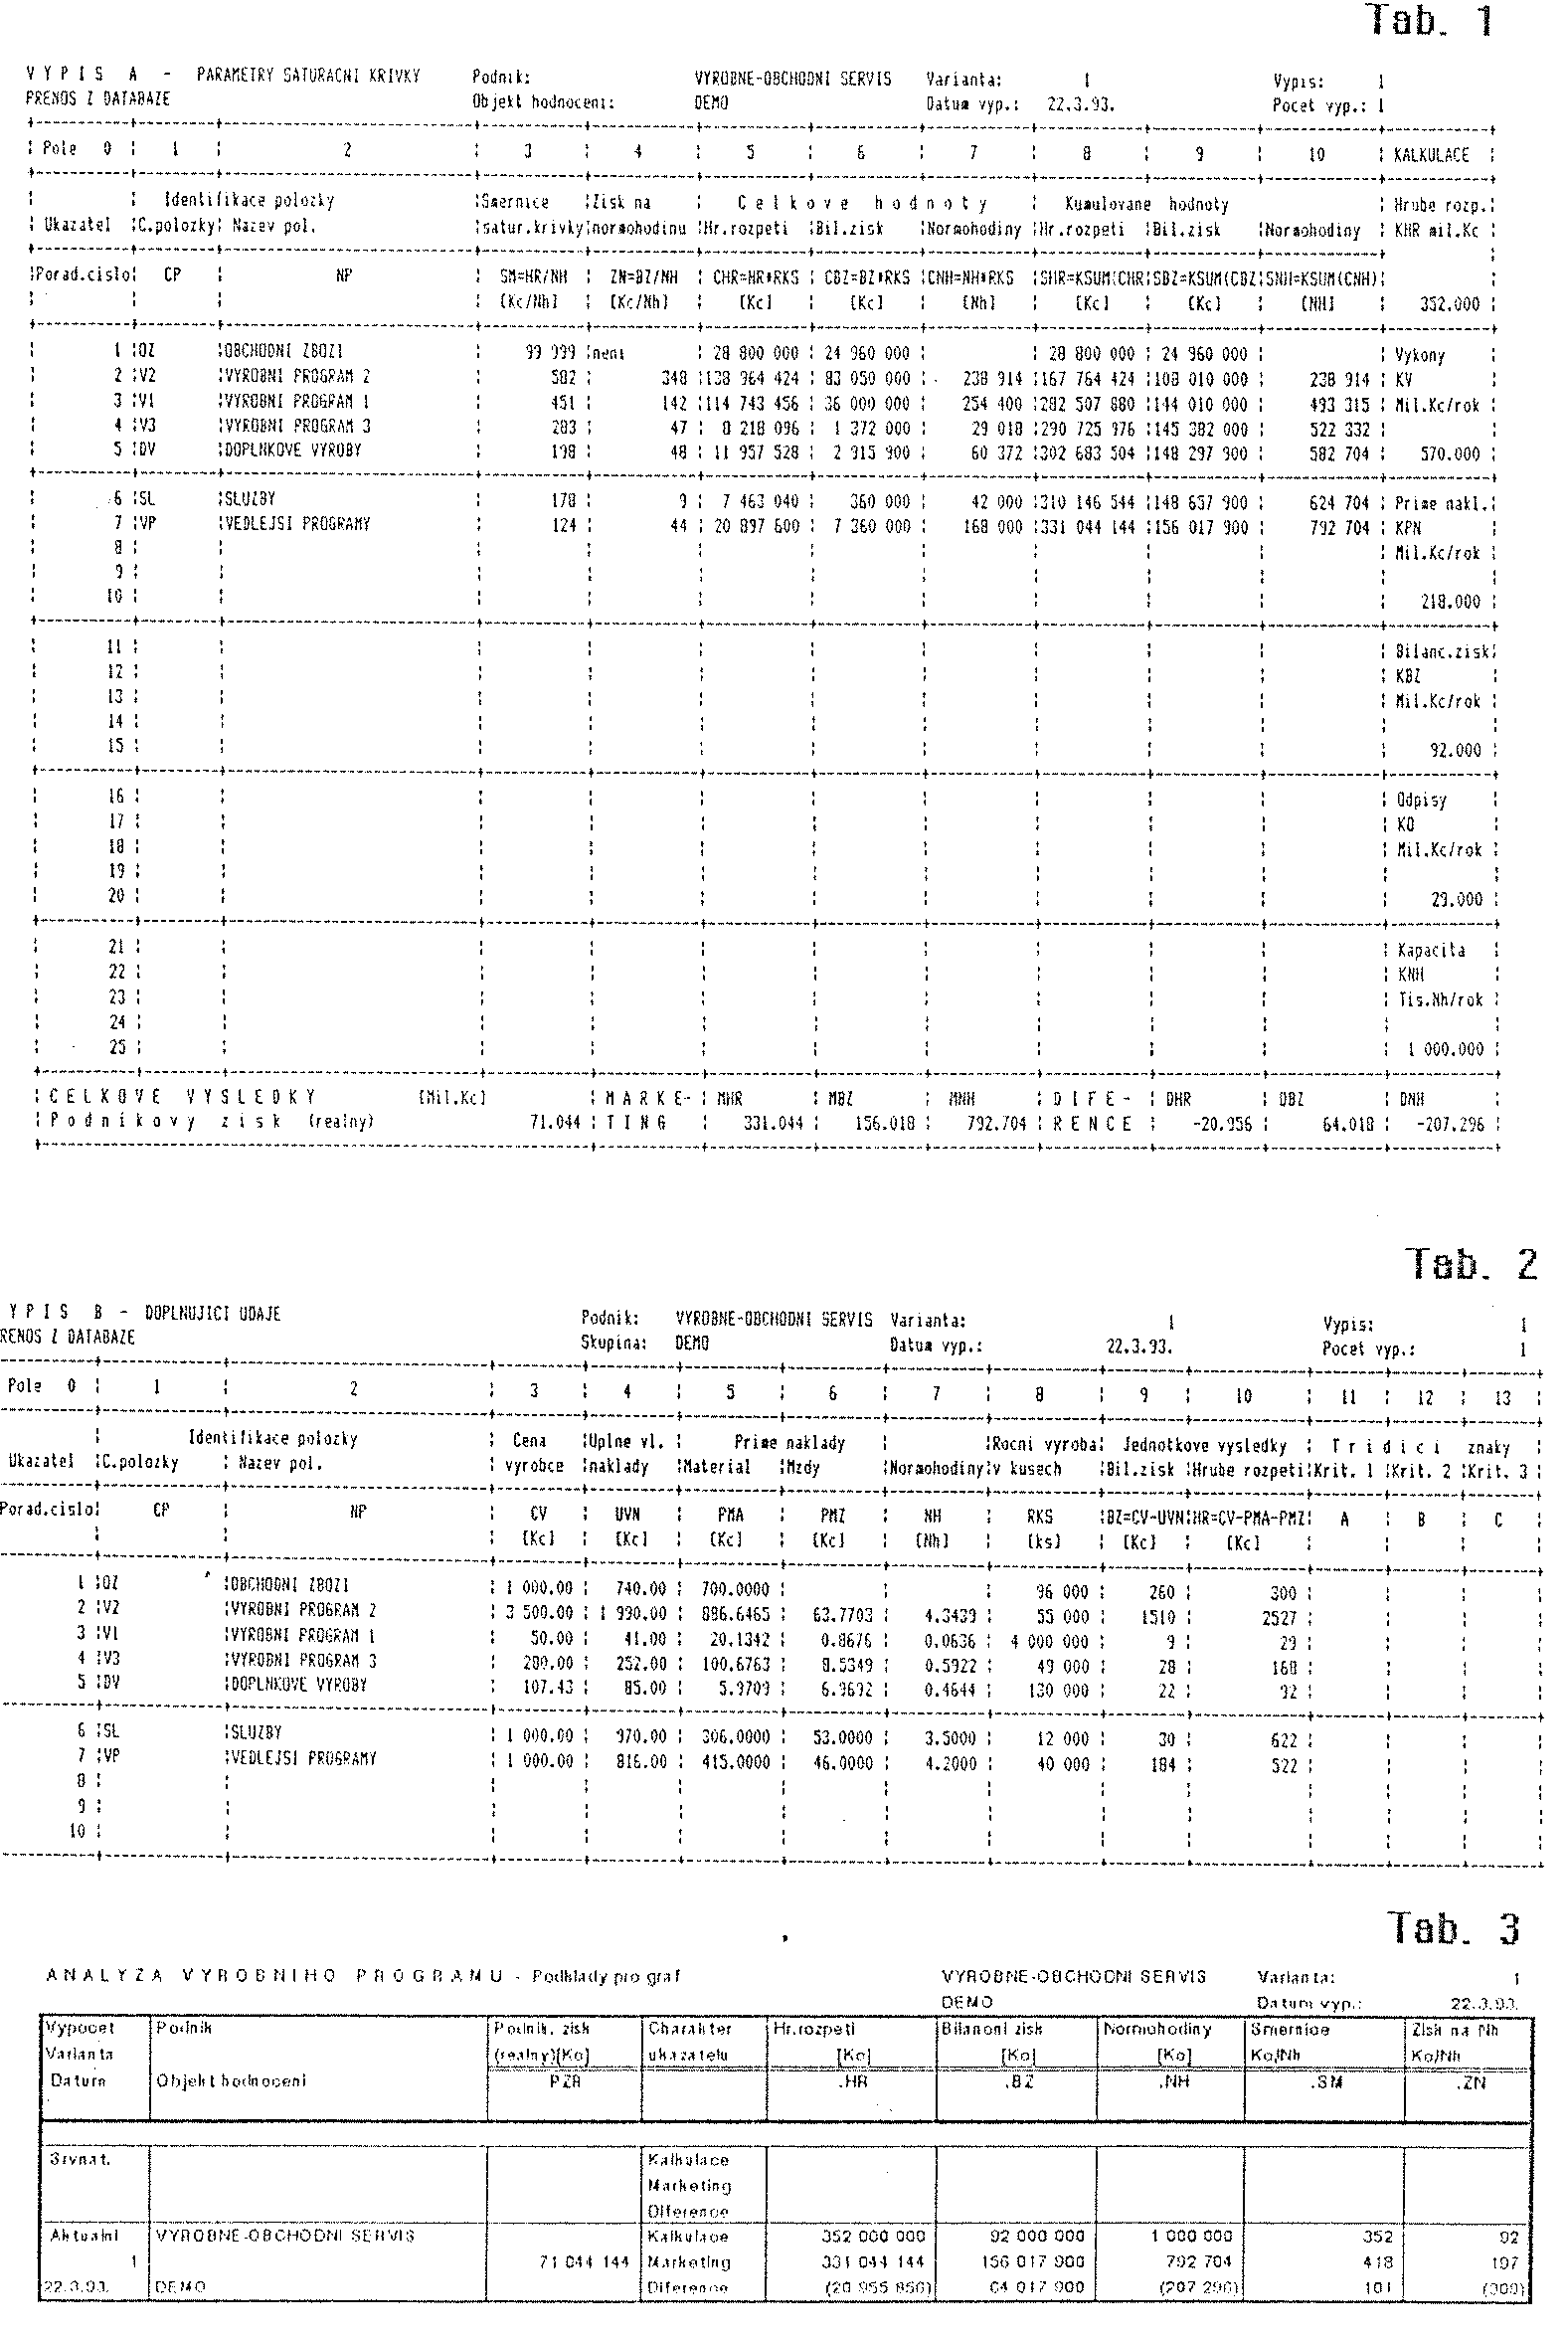
\includegraphics[width=\textwidth,height=\textheight,keepaspectratio]{./saturace-tab.png}

\newpage

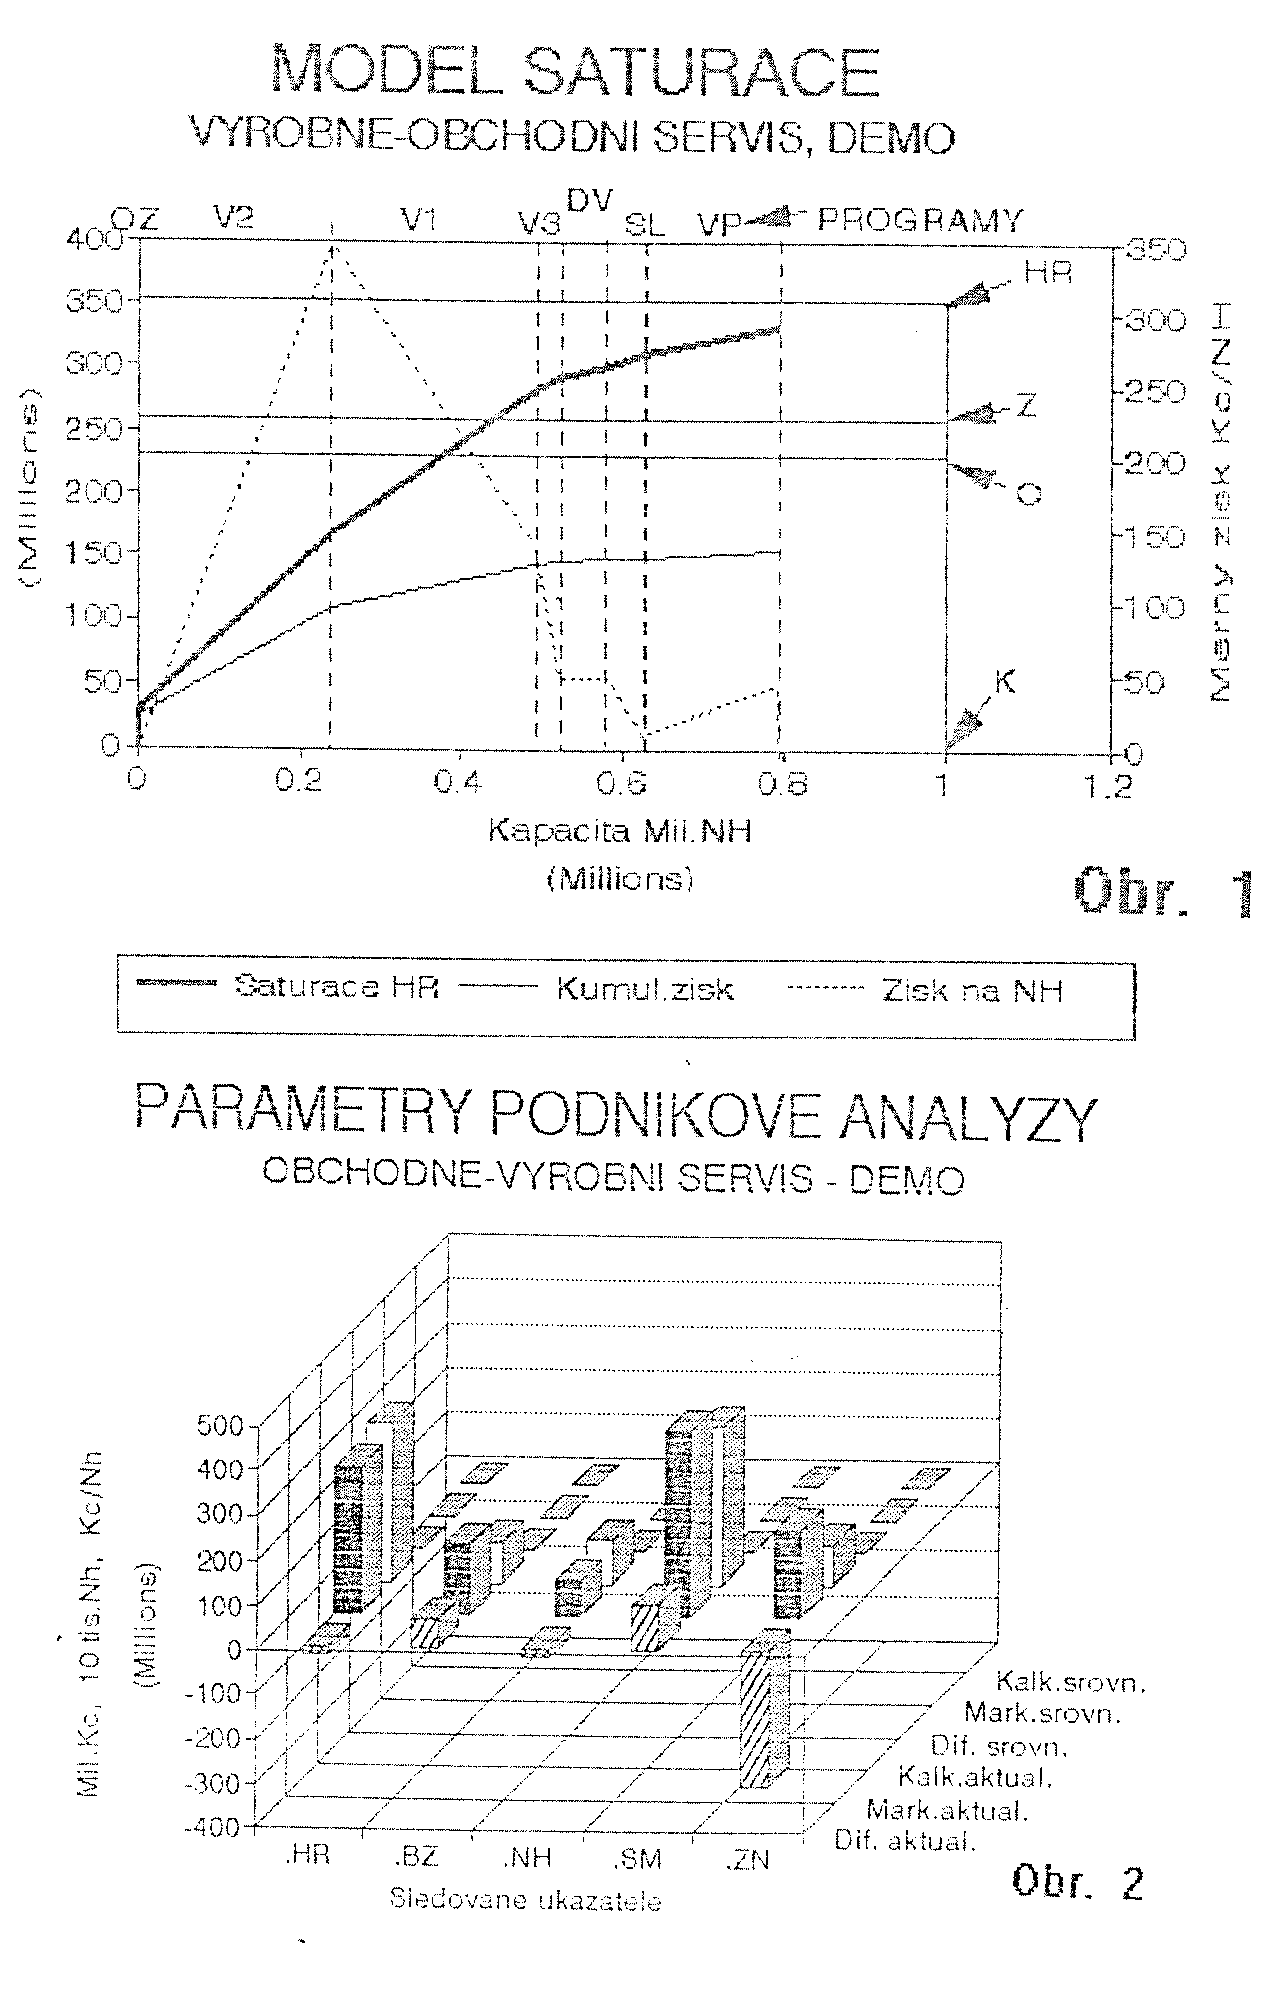
\includegraphics[width=\textwidth,height=\textheight,keepaspectratio]{./saturace-obr.png}


\end{document}
